\documentclass[aspectratio=169,11pt]{beamer}
\usepackage[T1]{fontenc}
\usepackage{lmodern}
\usepackage{amsmath,amssymb,mathtools,graphicx,tikz,booktabs,array}
\usetikzlibrary{arrows.meta,positioning}
\definecolor{Ink}{HTML}{162033}
\definecolor{Muted}{HTML}{657084}
\definecolor{Accent}{HTML}{2364AA}
\definecolor{Teal}{HTML}{148F88}
\definecolor{Paper}{HTML}{F7F8FA}
\definecolor{Warm}{HTML}{E08E0B}
\setbeamercolor{normal text}{fg=Ink,bg=Paper}
\setbeamercolor{structure}{fg=Accent}
\setbeamercolor{frametitle}{fg=Ink,bg=Paper}
\setbeamercolor{title}{fg=Ink}
\setbeamercolor{subtitle}{fg=Accent}
\setbeamercolor{author}{fg=Muted}
\setbeamercolor{date}{fg=Muted}
\setbeamerfont{title}{size=\fontsize{30}{34}\selectfont,series=\bfseries}
\setbeamerfont{subtitle}{size=\fontsize{16}{19}\selectfont}
\setbeamerfont{frametitle}{size=\fontsize{20}{24}\selectfont,series=\bfseries}
\setbeamertemplate{navigation symbols}{}
\setbeamertemplate{headline}{}
\setbeamertemplate{footline}{\leavevmode\hbox{%
\begin{beamercolorbox}[wd=.88\paperwidth,ht=2.8ex,dp=1.2ex,leftskip=.055\paperwidth]{author in head/foot}\color{Muted}\scriptsize nnActive \enspace | \enspace L\"uth et al., TMLR 2025\end{beamercolorbox}%
\begin{beamercolorbox}[wd=.12\paperwidth,ht=2.8ex,dp=1.2ex,center]{author in head/foot}\color{Muted}\scriptsize\insertframenumber\end{beamercolorbox}}}
\setbeamertemplate{frametitle}{\vspace{0.35cm}\hspace{0.2cm}\insertframetitle\par\vspace{0.08cm}}
\setbeamertemplate{itemize item}{\color{Accent}\small$\bullet$}
\setbeamersize{text margin left=0.8cm,text margin right=0.8cm}
\setlength{\parindent}{0pt}
\graphicspath{{figures/}}
\newcommand{\source}[1]{\vfill{\color{Muted}\fontsize{7}{9}\selectfont #1\par}}
\newcommand{\takeaway}[1]{\vspace{0.2cm}\begin{center}{\color{Accent}\large\bfseries #1}\end{center}}
\tikzset{flow/.style={-{Stealth[length=2mm]},draw=Muted,line width=.8pt},box/.style={fill=Accent!8,rounded corners=3pt,align=center,inner sep=9pt,font=\small}}
\title{nnActive}
\subtitle{\texorpdfstring{A Framework for Evaluation of Active Learning\\in 3D Biomedical Segmentation}{A Framework for Evaluation of Active Learning in 3D Biomedical Segmentation}}
\author{Carsten T. L\"uth et al.}
\date{Advanced Topics in Deep Learning \enspace | \enspace October 8, 2026}
\begin{document}

% Main talk: 16 slides, approximately 15 minutes. Backup slides follow.
{\setbeamertemplate{footline}{}
\begin{frame}[plain]
\vspace{0.55cm}\titlepage
\vspace{0.25cm}\centering{\color{Teal}\large Does active learning save annotation effort?}
\end{frame}}

\begin{frame}{The argument in four steps}
\vspace{0.4cm}
\begin{columns}[T,onlytextwidth]
\column{.23\textwidth}{\color{Accent}\Huge\bfseries 1}\par\vspace{.3cm}\textbf{The problem}\par\vspace{.2cm}\small Expensive labels\\Weak evaluation\\What should be compared?
\column{.23\textwidth}{\color{Accent}\Huge\bfseries 2}\par\vspace{.3cm}\textbf{The framework}\par\vspace{.2cm}\small Partial 3D labels\\Ensemble uncertainty\\Greedy vs. noisy selection
\column{.23\textwidth}{\color{Accent}\Huge\bfseries 3}\par\vspace{.3cm}\textbf{The evidence}\par\vspace{.2cm}\small Strong random baselines\\Four datasets\\Different winners
\column{.23\textwidth}{\color{Accent}\Huge\bfseries 4}\par\vspace{.3cm}\textbf{The interpretation}\par\vspace{.2cm}\small Accuracy vs. effort\\Ablations\\Limits and takeaway
\end{columns}
\takeaway{The baseline and the cost model can change the verdict.}
\end{frame}

\begin{frame}{Which part of a scan should we label next?}
\begin{columns}[c,onlytextwidth]
\column{.43\textwidth}
\textbf{Task:} assign an organ or tumor label to each voxel in a CT or MRI volume.
\vspace{.25cm}
\begin{itemize}\setlength{\itemsep}{7pt}
\item Expert delineation is expensive.
\item Nearby regions are redundant.
\item Much of the volume is background.
\end{itemize}
\column{.53\textwidth}\centering
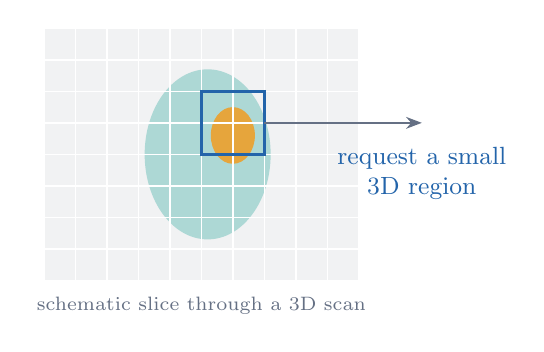
\begin{tikzpicture}[scale=.8]
\fill[Ink!6] (0,0) rectangle (5,4);
\fill[Teal!35] (2.6,2) ellipse (1.0 and 1.35);
\fill[Warm!80] (3,2.3) ellipse (.35 and .45);
\draw[step=.5,white,line width=.5pt] (0,0) grid (5,4);
\draw[Accent,line width=1.2pt] (2.5,2) rectangle (3.5,3);
\draw[flow] (3.5,2.5) -- (6,2.5);
\node[align=center,text=Accent,font=\small] at (6,1.7) {request a small\\3D region};
\node[text=Muted,font=\scriptsize] at (2.5,-.4) {schematic slice through a 3D scan};
\end{tikzpicture}
\end{columns}
\takeaway{Active learning lets the model choose the next annotation.}
\source{nnActive, Introduction and \S4. Illustration is schematic.}
\end{frame}

\begin{frame}{Four pitfalls in evaluating active learning}
\small\renewcommand{\arraystretch}{1.65}
\begin{tabular}{p{.43\linewidth}p{.49\linewidth}}
\textbf{What can go wrong?} & \textbf{nnActive's response}\\\midrule
Too few datasets or budgets & Four datasets, three budgets, repeated runs\\
Partial labels discard 3D context & 3D nnU-Net with a masked training loss\\
Random patches mostly hit background & Foreground-aware random baselines\\
Equal voxel counts hide unequal effort & Measure annotated foreground as well\\
\end{tabular}
\takeaway{A benchmark and evaluation framework,\\rather than a new segmentation architecture.}
\source{nnActive, \S3 and Figure 1.}
\end{frame}

\begin{frame}{The acquisition loop}
\centering\vspace{.25cm}
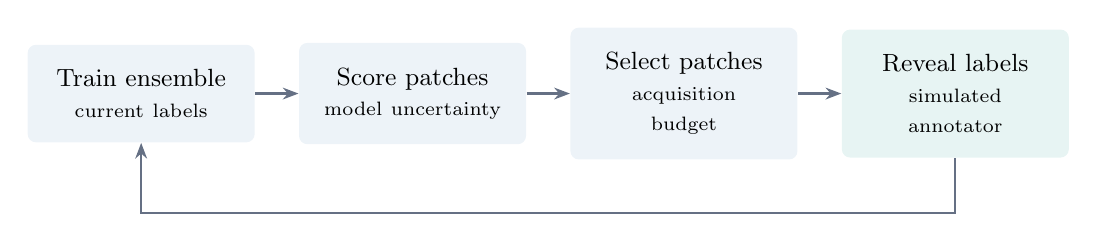
\begin{tikzpicture}[node distance=.55cm]
\node[box,text width=2.25cm] (train) {Train ensemble\\\scriptsize current labels};
\node[box,text width=2.25cm,right=of train] (score) {Score patches\\\scriptsize model uncertainty};
\node[box,text width=2.25cm,right=of score] (select) {Select patches\\\scriptsize acquisition budget};
\node[box,fill=Teal!10,text width=2.25cm,right=of select] (label) {Reveal labels\\\scriptsize simulated annotator};
\draw[flow] (train) -- (score);\draw[flow] (score) -- (select);\draw[flow] (select) -- (label);
\draw[flow] (label.south) -- ++(0,-.7) -| (train.south);
\end{tikzpicture}
\vspace{.65cm}
\begin{columns}[T,onlytextwidth]
\column{.48\textwidth}\textbf{Strong segmentation backbone}\par\small Five 3D full-resolution nnU-Net models, trained via five-fold cross-validation.\par\vspace{.18cm}200 epochs per model; retrain from scratch.
\column{.48\textwidth}\textbf{Shared acquisition protocol}\par\small Voxel scores averaged over query patches.\par\vspace{.18cm}No overlap with previously selected patches. Starting labels cover every foreground class.
\end{columns}
\source{nnActive, \S4--5.1. Ground-truth labels are revealed to simulate annotation.}
\end{frame}

\begin{frame}{A small annotation can use a larger context}
\begin{columns}[c,onlytextwidth]
\column{.47\textwidth}\centering
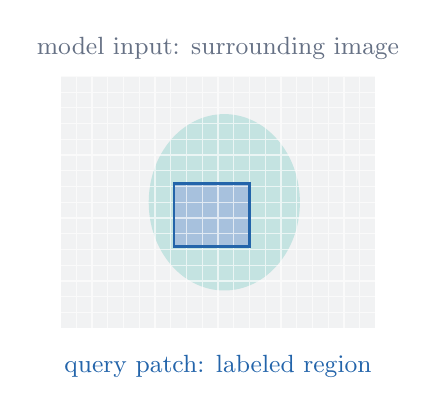
\begin{tikzpicture}[scale=.8]
\fill[Ink!6] (0,0) rectangle (5,4);
\fill[Teal!25] (2.6,2) ellipse (1.2 and 1.4);
\fill[Accent!40] (1.8,1.3) rectangle (3,2.3);
\draw[step=.25,white,opacity=.65] (0,0) grid (5,4);
\draw[Accent,line width=1pt] (1.8,1.3) rectangle (3,2.3);
\node[text=Muted,font=\small] at (2.5,4.45) {model input: surrounding image};
\node[text=Accent,font=\small] at (2.5,-.6) {query patch: labeled region};
\end{tikzpicture}
\column{.49\textwidth}
\textbf{Image context is available everywhere.}\par\vspace{.2cm}
Supervision is available only on the labeled voxel set $S$:
\[\mathcal L(\theta)=\sum_{v\in S}\ell\bigl(f_\theta(X)_v,Y_v\bigr).\]
\small Unlabeled voxels are ignored by the loss.\par\vspace{.25cm}
Region sampling varies the labeled voxel's position inside the model input.
\end{columns}
\takeaway{Query size and model input size are different.}
\source{nnActive, Appendix C.3. Equation illustrates the supervision mask, not the full nnU-Net loss.}
\end{frame}

\begin{frame}{Uncertain predictions or disagreement?}
\small For $M$ models, $\bar p(c\mid x)=\frac1M\sum_m p_m(c\mid x)$.
\vspace{.2cm}
\begin{columns}[T,onlytextwidth]
\column{.48\textwidth}
{\color{Accent}\large\textbf{Predictive Entropy}}
\[H(\bar p)=-\sum_c\bar p_c\log\bar p_c\]
Select patches with uncertain average predictions.
\column{.48\textwidth}
{\color{Teal}\large\textbf{BALD}}
\[H(\bar p)-\frac1M\sum_m H(p_m)\]
Select patches where ensemble members disagree.
\end{columns}
\vspace{.35cm}\small\renewcommand{\arraystretch}{1.35}
\begin{tabular}{p{.59\linewidth}cc}
\textbf{Binary example, same mean prediction} & \textbf{Entropy} & \textbf{BALD}\\\midrule
Every model predicts $(0.5,0.5)$ & High & Zero\\
Half predict $(1,0)$, half $(0,1)$ & High & High\\
\end{tabular}
\source{nnActive, \S4 and Appendix C. Ensemble BALD approximates Bayesian model disagreement.}
\end{frame}

\begin{frame}{Why add noise to patch selection?}
\begin{columns}[T,onlytextwidth]
\column{.48\textwidth}
{\color{Accent}\large\textbf{Greedy selection}}\par\vspace{.25cm}
Take the highest uncertainty scores.\par\vspace{.2cm}
\begin{itemize}\item Predictive Entropy\item BALD\end{itemize}
\vspace{.2cm}Risk: many selected patches may look alike, even without spatial overlap.
\column{.48\textwidth}
{\color{Teal}\large\textbf{Noisy selection}}\par\vspace{.25cm}
Perturb scores or ranks before selecting.\par\vspace{.2cm}
\begin{itemize}\item PowerPE\item PowerBALD\item SoftrankBALD\end{itemize}
\vspace{.2cm}Randomness can broaden selection, especially when labels are scarce.
\end{columns}
\takeaway{Highest uncertainty does not guarantee the best batch.}
\source{nnActive, \S4 and \S5.2. Randomized selection does not guarantee semantic diversity. Main study: $\beta=1$.}
\end{frame}

\begin{frame}{A benchmark across tasks and budgets}
\small\renewcommand{\arraystretch}{1.35}
\begin{tabular}{lp{.43\linewidth}r}
\textbf{Dataset} & \textbf{Segmentation targets} & \textbf{Low / medium / high}\\\midrule
ACDC & Three cardiac structures, MRI & 150 / 300 / 450\\
AMOS2022 & Fifteen organs & 200 / 1,000 / 2,500\\
KiTS2021 & Kidney, tumor and cyst & 200 / 1,000 / 2,500\\
Hippocampus & Anterior and posterior regions & 100 / 200 / 300\\\bottomrule
\end{tabular}\par
\vspace{.15cm}{\color{Muted}\scriptsize Budgets are numbers of query patches; patch dimensions depend on the dataset.\par}
\vspace{.35cm}
\begin{columns}[T,onlytextwidth]
\column{.49\textwidth}\textbf{Matched comparisons}\par\small 75\% training/acquisition pool; 25\% test.\\Eight methods; four acquisition seeds.
\column{.47\textwidth}\textbf{Five budget points}\par\small 20\%, 40\%, 60\%, 80\%, 100\%.\\Shared initial labels; four further acquisitions.
\end{columns}
\source{nnActive, \S5.1 and Appendix E. More than 7,500 model trainings including ablations.}
\end{frame}

\begin{frame}{Foreground-aware random sampling}
\begin{columns}[T,onlytextwidth]
\column{.40\textwidth}
{\color{Accent}\large\textbf{Uniform Random}}\par\vspace{.25cm}
Choose patches anywhere in the volume.\par\vspace{.25cm}
Many queries can land on easy background.
\column{.56\textwidth}
{\color{Teal}\large\textbf{Random 66\% FG}}\par\vspace{.25cm}
Approximately one-third of queries are uniform. Two-thirds target foreground:\par
\begin{itemize}\item Half centered on a sampled foreground class.\item Half centered on a class boundary.\end{itemize}
\end{columns}
\takeaway{Can uncertainty selection beat cheap,\\anatomy-aware sampling?}
\source{nnActive, \S4. Random 33\% FG uses the same mechanism less often. Ground truth simulates localization; real screening cost is unmeasured.}
\end{frame}

\begin{frame}{The baseline changes the verdict}
\centering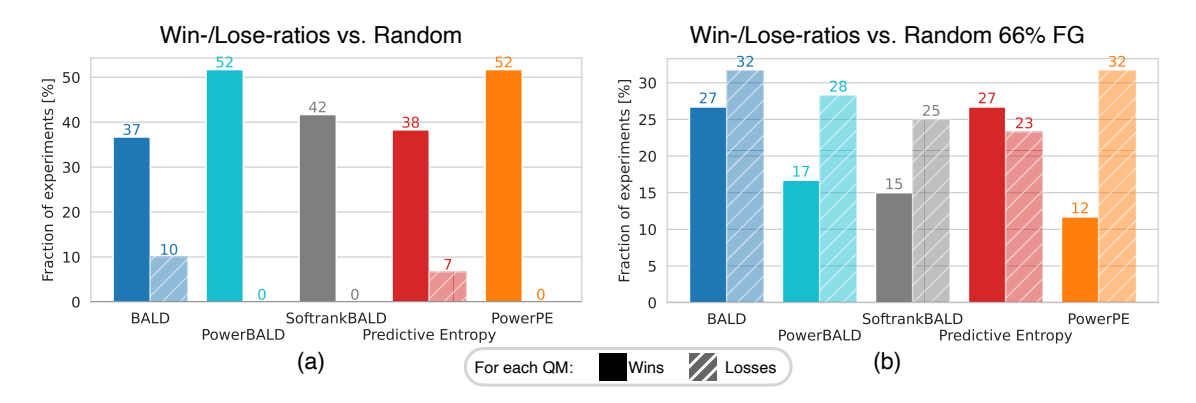
\includegraphics[width=.97\linewidth]{wins.png}
\vspace{.1cm}\small
Against uniform Random: many more wins than losses.\par
Against Random 66\% FG: only Predictive Entropy has a positive win/loss balance.
\source{nnActive, Figure 3. Bars show significant pairwise wins/losses across comparisons ($t$-tests, $\alpha=.05$), not Dice gains.}
\end{frame}

\begin{frame}{The dataset can reverse the winner}
\small\renewcommand{\arraystretch}{1.5}
\begin{tabular}{lrrr}
\textbf{Final Dice $\times100$} & \textbf{Random} & \textbf{Random 66\% FG} & \textbf{Entropy}\\\midrule
AMOS, low budget & 36.36 & {\color{Teal}\textbf{71.11}} & 39.19\\
KiTS, medium budget & 48.41 & 51.67 & {\color{Accent}\textbf{65.39}}\\\bottomrule
\end{tabular}
\vspace{.45cm}
\begin{columns}[T,onlytextwidth]
\column{.48\textwidth}{\color{Teal}\large\textbf{AMOS: cover all organs}}\par\vspace{.2cm}\small Foreground-aware sampling covers small structures. Greedy uncertainty can focus repeatedly on a subset of classes.
\column{.48\textwidth}{\color{Accent}\large\textbf{KiTS: learn difficult background}}\par\vspace{.2cm}\small Uncertainty selection can target background regions causing false positives. Foreground sampling can miss them.
\end{columns}
\source{nnActive, Table 6 and \S5.2 Q4. Compare within rows. Values are reported means; explanations are the authors' interpretations.}
\end{frame}

\begin{frame}{Measuring annotation effort}
\begin{columns}[c,onlytextwidth]
\column{.55\textwidth}\centering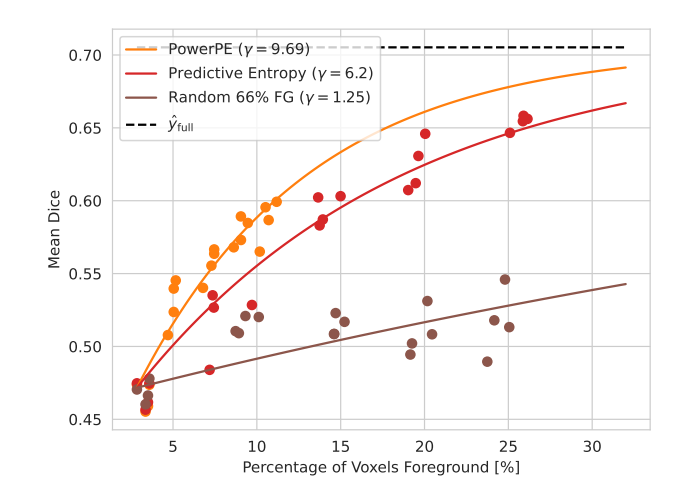
\includegraphics[width=\linewidth]{foreground-efficiency.png}
\column{.41\textwidth}\small
\textbf{Foreground Efficiency}\par\vspace{.15cm}
Fit how quickly the gap to fully labeled performance closes as annotated foreground increases. Larger $\gamma$ means faster closure.\par\vspace{.25cm}
\textbf{KiTS, medium budget}\par
PowerPE: $\gamma=9.69$, Dice $58.67$.\\
Entropy: $\gamma=6.20$, Dice $65.39$.\par\vspace{.25cm}
Better efficiency can coexist with lower final accuracy.
\end{columns}
\source{nnActive, Figure 7 and Table 6. Foreground count is a proxy for human effort. Compare $\gamma$ only within matched setups.}
\end{frame}

\begin{frame}{What changes the acquisition outcome?}
\small\renewcommand{\arraystretch}{1.55}
\begin{tabular}{p{.29\linewidth}p{.63\linewidth}}
\textbf{Ablation} & \textbf{Finding and trade-off}\\\midrule
Smaller acquisition batches & More frequent feedback generally helps, but requires more retraining and inference.\\
Longer training & Better-trained models also select better patches; the gain is not only better final fitting.\\
More selection noise & Often helps at low budgets; less noise can help later. No universal best setting.\\
Smaller query patches & Relative method rankings change. Halving each dimension labels eight times fewer voxels per patch.\\
\end{tabular}
\source{nnActive, \S5.3 and Appendix G. Smaller patches do not establish equal accuracy with eight times less annotation.}
\end{frame}

\begin{frame}{How far should we trust the conclusion?}
\begin{columns}[T,onlytextwidth]
\column{.48\textwidth}
{\color{Teal}\large\textbf{Strong evidence}}\par\vspace{.2cm}
\begin{itemize}\setlength{\itemsep}{8pt}
\item Strong 3D segmentation pipeline.
\item Diverse tasks, budgets and seeds.
\item Stronger baselines and cost proxies.
\end{itemize}
\column{.48\textwidth}
{\color{Accent}\large\textbf{Remaining assumptions}}\par\vspace{.2cm}
\begin{itemize}\setlength{\itemsep}{8pt}
\item Foreground localization is simulated with ground truth.
\item Foreground voxels do not measure annotation minutes.
\item Five uncertainty methods do not cover all active learning.
\end{itemize}
\end{columns}
\takeaway{Structured starting labels already cover every class.\\The study does not test a fully unlabeled cold start.}
\source{nnActive, \S4--6 and Appendix D.4.}
\end{frame}

\begin{frame}{Does active learning save annotation effort?}
\vspace{.25cm}
\begin{enumerate}\setlength{\itemsep}{15pt}
\item It usually beats \textbf{uniform random} patch sampling.
\item No tested method consistently dominates \textbf{foreground-aware random} sampling across tasks and budgets.
\item \textbf{Predictive Entropy} is strongest among the active methods overall; early performance and effort still matter.
\end{enumerate}
\takeaway{Show gains over a strong baseline\\under a defensible annotation-cost model.}
\vspace{.1cm}\centering{\color{Muted}\small Questions}
\source{nnActive, \S5.2 and \S6. Random 66\% FG has the best mean AUBC rank in the main study.}
\end{frame}

\appendix
\begin{frame}{Backup: interpreting the metrics}
\small\renewcommand{\arraystretch}{1.5}
\begin{tabular}{p{.24\linewidth}p{.68\linewidth}}
\textbf{Final Dice} & Accuracy at the final budget point. Dice: $2|P\cap G|/(|P|+|G|)$.\\
\textbf{AUBC} & Area under the budget curve: performance throughout acquisition, including early budgets.\\
\textbf{PPM} & Frequency of significant pairwise wins. Does not show the size of improvements.\\
\textbf{FG-Eff} & Fitted rate of convergence per fraction of foreground annotated, under matched training and initialization.\\
\end{tabular}
\vspace{.25cm}\[y(t)=(\hat y(\hat t_0)-\hat y_{\mathrm{full}})e^{-\gamma(t-\hat t_0)}+\hat y_{\mathrm{full}}.\]
\source{nnActive, Appendix D. $t$: annotated foreground fraction; $\hat t_0$: initial fraction; $\hat y_{\mathrm{full}}$: matched full-data reference.}
\end{frame}

\begin{frame}{Backup: noise strength and budget}
\begin{columns}[c,onlytextwidth]
\column{.60\textwidth}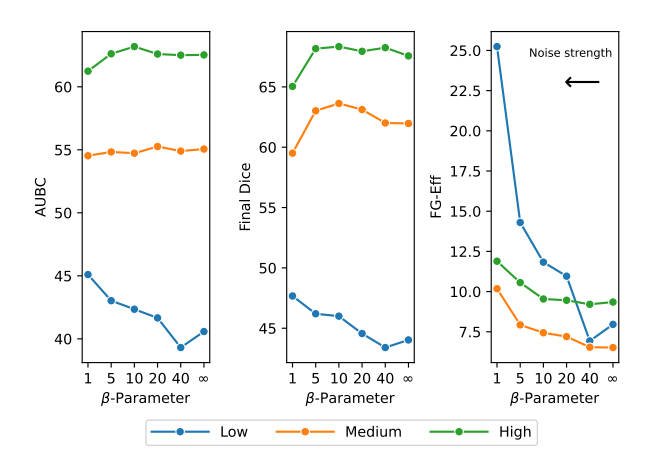
\includegraphics[width=\linewidth]{noise-ablation.png}
\column{.36\textwidth}\small
\[s'=\log(s_{\mathrm{BALD}})+\epsilon\]
\[\epsilon\sim\mathrm{Gumbel}(0,\beta^{-1})\]
Larger $\beta$ means less noise.\par\vspace{.2cm}
$\beta\to\infty$ approaches greedy BALD.\par\vspace{.2cm}
On KiTS, strong noise is particularly valuable at low budgets.
\end{columns}
\source{nnActive, Figure 5 and Appendix G.3. Curves are specific to KiTS; they do not define a universal schedule.}
\end{frame}

\begin{frame}{Backup: source and scope}
\textbf{Carsten T. L\"uth et al. (2025)}\par\vspace{.15cm}
\emph{nnActive: A Framework for Evaluation of Active Learning in 3D Biomedical Segmentation.}\par\vspace{.15cm}
Transactions on Machine Learning Research, August 2025.
\vspace{.35cm}
\begin{itemize}\setlength{\itemsep}{9pt}
\item Results and figures use the course's August 2025 PDF.
\item Main results: \S5.2, Figures 3--4, Appendix F / Table 6.
\item Cost metric: Appendix D.4 / Figure 7.
\item Ablations: \S5.3 and Appendix G.
\end{itemize}
\vspace{.25cm}\small
\href{https://openreview.net/forum?id=AJAnmRLJjJ}{Published paper: openreview.net/forum?id=AJAnmRLJjJ}\par
\href{https://arxiv.org/abs/2511.19183}{Later arXiv version: arxiv.org/abs/2511.19183}
\end{frame}
\end{document}
